\chapter{Evaluation}
\label{evaluation}

In this chapter, CCDetect-LSP will be evaluated based on different criteria, which combined
will provide a basis for evaluating the tool as a whole.

First, we will verify that CCDetect-LSP correctly identifies type-1 clones. We will use
the BigCloneBench~\cite{BigCloneBench} database and BigCloneEval~\cite{BigCloneEval} tool,
which is the standard tools used to test clone detection accuracy.

Since the tool is focused on efficient detection of code clones, real-time performance of
the tool will be a high priority in its evaluation. We will compare the time of the
initial detection with the incremental updates. Note that we will also distinguish between
the initial detection where parsing the entire code base is necessary, and subsequent
detections which still constructs the suffix array from scratch, but does not require
parsing the entire code base. We will call this type of detection the SACA detection,
while the detection which uses the dynamic extended suffix arrays will be called the
incremental detection. This is done to compare the dynamic extended suffix array against
building the suffix array from scratch. Performance will be evaluated in two ways:

\begin{itemize}
    \item Informal complexity analysis of phases in initial, SACA and incremental detection
    \item Performance benchmark of initial, SACA and incremental detection
    \item Performance benchmark comparison with iClones~\cite{GodeIncrementalCloneDetection}
\end{itemize}

\section{Verifying clones with BigCloneBench}

In order to verify that CCDetect-LSP correctly identifies clones, we should analyze and
confirm that CCDetect-LSP finds all clones in a given code base.
BigCloneBench~\cite{BigCloneBench} is a clone detection benchmark of a set of known clones
in a dataset called ``IJaDataset''. The benchmark consists of the IJaDataset and a
database containing information of the clones which exist in the dataset.
BigCloneEval~\cite{BigCloneEval} is a tool which simplifies evaluation of a tool on the
BigCloneBench. BigCloneEval evaluates a tool by running the tool on the dataset, letting
the tool output all the clones the tool finds, and then matching the clones the tool found
with the clones in the database. The clones in the database are manually verified by
humans, and include type-1 to type-3 clones.

We evaluated CCDetect-LSP by running the initial detection algorithm on the dataset, and
outputting all the clones the tool found. BigCloneEval expects to get a file where each
line contains a clone pair, where a clone is specified with filename, starting and
ending line. This was simple to extract from our clone-map, where we converted our ranges
which point to the beginning and ending token, to just the line number of those tokens.

BigCloneEval reports the recall of a tool, meaning the percentage of found clones.
Therefore, we did not make sure that our conversion to the format BigCloneEval expects
gave the minimum number of clone pairs. For example, for a clone pair of clones $A$ and
$B$, we output both that $A$ is a clone of $B$ and that $B$ is a clone of $A$, which is
superfluous. This would lead to a bad precision, but does not affect the recall in the
report which BigCloneEval outputs.

We used the following command and parameters to evaluate CCDetect-LSP:
$$
\text{./evaluateTool --min-tokens=100 -s=100 --output=ccdetect.report -t=1 }
$$

For CCDetect-LSP, we used mostly the default parameters of BigCloneEval, but we increased
the minimum clone size to $100$ and set the minimum similarity threshold to be $100\%$,
since we are only evaluating CCDetect-LSP for type-1 clone recall. This was done to reduce
the time an evaluation takes as it does not consider type-3 clones when the similarity
threshold is set to $100\%$, and the default token threshold of $50$ requires a lot of
time to match clones with the database.

Appendix \ref{bcblog} shows the beginning of the report generated by BigCloneEval when
CCDetect-LSP is evaluated. The report shows that CCDetect-LSP has a $~99.98\%$ recall for
type-1 clones. CCDetect-LSP is clearly capable of detecting type-1 clones. As for the
missing type-1 clones, while it is not so simple to determine which clones were not
detected, it is possible that these clones are not reported because of inconsistencies in
the database. The report also shows that CCDetect-LSP manages to detect a few type-2
clones. Detecting these are accidental, as CCDetect-LSP does not currently implement any
normalization of the input which would allow for type-2 detection. These type-2 clones are
likely detected because BigCloneEval allows some leniency in terms of how much a clone
reported by CCDetect-LSP needs to match with a clone reported in the BigCloneBench
database. Therefore, it is likely the case that a few type-2 clones overlap with a type-1
clone, and BigCloneEval matched these clones because of its leniency.

\section{Time complexity of detection}

In this section we will conduct an informal analysis of the running time of each phase of
the initial, SACA and incremental detection to argue that the average runtime complexity
of the incremental detection is more efficient than the initial detection. In each phase
we will argue the run time in terms of Big O notation. Some claims will be substantiated
in the next section where we look at concrete code bases and their properties.

The initial detection runs in $O(n)$ time, where $n$ is the number of characters in the
code base. The bottleneck of the initial detection is reading and parsing all the content
in each file. Tree-sitter generates Generalized LR (GLR) parsers~\cite{GLR}, which in the
worst-case have a $O(n^3)$ running time, but $O(n)$ for any deterministic grammar. As
programming languages generally have deterministic grammars, we will assume that the
running time of parsing with Tree-sitter takes $O(n)$ time. After the initial parsing, the
SACA detection runs in $O(f)$ time, where $f$ is the size of the fingerprint and $f \ll
n$. The running time is $O(f)$ because the suffix array construction is performed for
every update, which takes linear time in the size of the input, which is the fingerprint.
The extraction of clones from the LCP array also runs in $O(f)$ as it is a single scan
over the LCP array. The final source-mapping is a bit more complicated, taking
$O(\vert\text{clones}\vert \times \log (\vert\text{documents}\vert))$. This complexity
comes from binary-searching the list of documents to find the correct document for each
clone. This is highly likely to be less time consuming than the suffix array construction,
as the number of documents and number of clones are usually orders of magnitude lower than
the size of the whole code base. Therefore, we get a final running time of $O(f) +
O(\vert\text{clones}\vert \times \log(\vert\text{document}\vert))$, where $O(f)$ is highly
likely to be the slowest factor.

For the incremental detection, we have already parsed the code base and built the index
and dynamic extended suffix array structure for the code base. Afterwards, when an edit
$E$ is performed in a document $D$, the first phase is to update the document index. We
iterate over the documents to update their fingerprint ranges, and when a document which
has been edited is reached, the new document content is incrementally re-parsed, queried
for fragments and then the fragments are fingerprinted. In the worst-case, we have to
fingerprint the entire document, which has a complexity of $O(\vert D\vert)$.

Next, extracting the edit operations which have happened to $D_f$ (fingerprint of $D$),
takes $O(\vert D_f\vert + \vert E\vert^2)$ where $\vert E\vert \leq \vert D_f\vert$. Note
that the size of the edit is calculated as the area which $E$ covers, meaning that if an
edit consists of changing a token at the beginning of the file, and a token at the end of
the file, then $\vert E\vert \approx \vert D_f\vert$. We get this time complexity because
Hirschberg's algorithm runs in $O(n \times m)$ where in our case, $n \approx m$. If the
size of the edit is contained in a smaller area, we apply the optimization which reduces
the size of the edit by comparing characters at the beginning and end of the string, as
discussed in \cref{dynamicdetection}. This process has a complexity of $O(\vert D\vert)$,
and afterwards Hirschberg's algorithm has a worst-case complexity of $O(\vert E\vert^2)$.

The worst-case complexity of dynamically updating the extended suffix array is actually
slower than a linear time SACA algorithm in the worst-case. The worst-case scenario when
inserting/deleting a character in the fingerprint is that every single suffix needs to be
reordered, meaning we reorder $O(f)$ suffixes, where each reordering takes $O(\log(f))$
time, as it requires deleting and inserting an element in the dynamic extended suffix
array. In addition, we need to call the LF function twice for each reordering, which has a
$O(\sigma + \log f \log\sigma)$ complexity. The complexity of the LF function comes from a
$rank$ call in the wavelet matrix, and an iteration over $C$ to find the number of smaller
characters. This results in a $O(f \times (\log f + \sigma + \log f \log\sigma))$ running
time of this phase, which is worse than the $O(f)$ running time of the SACA algorithm. In
addition, before the reordering when we are inserting/deleting characters in the BWT, we
use the LF function and insert/delete in the wavelet matrix and the $C$ array. The highest
complexity of these operations is again the LF function. If an edit operation consists of
inserting/deleting multiple characters, the number of LF function calls is increased, with
a complexity of $O(e \times (\sigma + \log f \log\sigma))$, where $e$ is the number of
characters inserted/deleted. Note that while there are many factors in this time
complexity, all the factors should be quite small compared to $f$, making the complexity of
reordering the suffixes the slowest factor of this phase.

The average-case complexity of this phase is however highly likely to be faster. Salson et
al.~\cite{DynamicExtendedSuffixArraysReorderings} have shown that on average, the number
of reorderings required for an insertion/deletion in a suffix array is highly correlated
with the average LCP value of the input. Their data shows that for multiple different
types of data such as genome sequences and english text, the average LCP value of the
input is generally magnitudes lower than the input size. In our experiments, this applies
to source code as well, as code bases we have tested on have all had an average LCP values
well below $100$. See table \ref{tab:codebases} to see the average LCP value for different
codebases. A lower number of reorderings for lower LCP values seems intuitive, as
lower LCP values mean that the insertion/deletion will affect the ordering of fewer
suffixes in the input. With this information, it would be more accurate to downplay the
importance of the $O(f)$ number of reorderings in our analysis, and we therefore claim
that the average running time of an edit operation on the suffix array is closer to $O(\log f +
(e \times \sigma + \log f \log\sigma))$. We extend this to account for multiple edit operations as
well, for each edit operations which was computed in the last phase, we perform an
insertion/deletion of $e$ characters. Therefore, the total complexity of this phase on
average is closer to $O(\vert\text{edits}\vert \times (\log f + (e \times \sigma + \log f
\log\sigma)))$.

Next there is the clone extraction phase. Recall that in the dynamic detection clone
extraction phase, we had stored all nodes with an LCP value above the token threshold, and
iterate over those to determine which of them are clones or not. In the worst-case, every
index in the LCP array would be above the token threshold, which would be an $O(f)$
complexity iteration. However, this is highly unlikely, since the nodes with LCP value
above the token threshold are either clones, or contained clones. The number of contained
clones is limited by the number of clones because each clone can only have a limited
amount of contained clones. Therefore, the number of LCP nodes examined should be closer
to $O(\vert\text{clones}\vert)$, which is highly likely to be much less expensive than
iterating over all the LCP nodes. For each examined LCP node, we need to traverse from the
node, to its pointer node, and then to the root of the $B$ tree to determine the
fingerprint index of that LCP node. We do the same to determine the index of the matching
clone, as described in \cref{dynamicdetection}. These traversals take $O(\log f)$ time.
The worst-case performance of this phase is therefore $O(f \times \log(f))$, but we will
see that the average-case performance is closer to $O(\vert\text{clones}\vert \times
\log(f))$.

Finally, the source-mapping phase is easier to analyze. As we now know all the positions
of clones and their matches, building the clone-map takes $O(\vert\text{clones}\vert
\times \log(\vert\text{documents}\vert))$ time. We perform the binary-search over the
documents to get the source location for each clone index we found in the previous phase.
This is the same complexity for both the SACA and incremental detection.

With this informal analysis, we have shown that in the average case, the incremental
detection should be faster than the SACA detection, as none of the phases reach or exceed
the $O(f)$ running time of the SACA detection. In the next section we will show that the
properties we have assumed for this analysis are present in multiple code bases, and that
these properties do lead to better performance for the incremental detection.

\section{Benchmark performance}

For the performance benchmark we will benchmark the running time of CCDetect-LSP on code
bases and edits of different sizes. We will compare the performance of the incremental
detection with the SACA detection and iClones~\cite{GodeIncrementalCloneDetection}.

iClones is a tool which similarly to CCDetect-LSP, does incremental clone detection. The
tool takes $n$ revisions of the same code base and will after the initial detection, reuse
as much information as possible to reduce the amount of work needed to analyze consecutive
revisions. The algorithm which iClones uses is based on generalized suffix trees (GST),
and the tool can detect up to type-3 clones. For a revision $i$, iClones excepts to have a
file named \verb|changed| in the root folder of the revision, which contains information
on which files have changed between revision $i - 1$ and $i$. For each file which has
changed, the suffixes in the file is inserted into the GST, reusing nodes of the tree if
possible.

For the performance benchmark, the code bases are set up in the way iClones expects. For
each code base to analyze, we will store $n$ revisions of it, where each revision contains
some changes to some of the files. An evaluation program for CCDetect-LSP was written so
that it can process this same setup, making it simple to run both CCDetect-LSP and iClones
on the same code bases, and compare their results.

For each code base, we can generate new revisions. Generating new revisions of a code base
means that we copy the code base and apply a few insertions/deletions to random files, to
simulate how a programmer would edit files when programming. Generating new revisions of
code bases is not a trivial problem, since each edit performed in a file should still give
a valid program which can be parsed. If the file cannot be parsed, Tree-sitter will not
give a proper AST for the file. Because of this, generating insertions is hard, because we
need to make sure that the location we are inserting some code is a valid location for
that code. It is easier to generate deletions first instead. Deletions are easier to
generate, as we can use Tree-sitter to determine where a fragment of size $n$ is located,
and remove that section of code in the next revision. For example in Java, we can delete
an entire method, and still know that the program will parse to a valid AST afterwards.
After we have generated for example $10$ revisions where the difference between each
revision is deletion of some number of fragments, we can then reverse the ordering of the
revisions, so that the final revision is now the first revision, and so on. This will
translate each deletion to instead be an insertion, as an insertion is simply an inversion
of a deletion. Figure \ref{fig:revisioninversion} show graphically how a test consisting
of three revisions with deletions can be inverted to create a test of insertions.

\begin{figure}[t]
    \begin{center}
        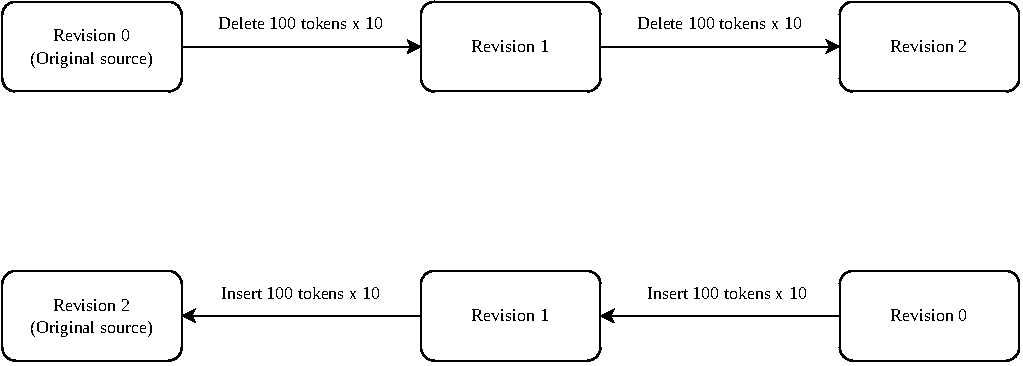
\includegraphics[width=0.95\textwidth]{figures/revisioninversion.drawio.pdf}
    \end{center}
    \caption{Reversion of an evaluation test. Delete100x10 to Insert100x10}
    \label{fig:revisioninversion}
\end{figure}

With this technique, generating an arbitrary amount of tests is now possible. There are
multiple variables we can tune when generating the tests. Primarily the three most
important factors of the tests is the size of the code base, the number of edit operations
in each revision, and the size of those edit operations.

The size of the code base will naturally affect the running time of the algorithm. We
randomly picked open-source code bases of differing sizes and differing amounts of
duplication to run the benchmark on. We selected the code bases
WorldWind\footnote{WorldWind: \url{https://github.com/NASAWorldWind/WorldWindJava}}, neo4j\footnote{neo4j:
\url{https://github.com/neo4j/neo4j}}, graal\footnote{graal:
\url{https://github.com/oracle/graal}}, flink\footnote{flink:
\url{https://github.com/apache/flink}}, elasticsearch\footnote{elasticsearch:
\url{https://github.com/elastic/elasticsearch}} and
intellij-community\footnote{intellij-community:
\url{https://github.com/JetBrains/intellij-community}}. The code bases chosen were
different size Java code bases, with different amounts of duplication. Table
\ref{tab:codebases} shows some properties of the code bases, including its number of
lines, the number of clones detected by CCDetect-LSP for a token threshold of $100$, the
average LCP value and the number of LCP values above $100$. An interesting aspect of the
graal and flink code bases is that they both contain $\sim2.2\text{MLOC}$, but graal has a
much higher $\text{LCP}_\text{avg}$, which could potentially lead to a slower suffix array
update.

\begin{table}[t]
    \begin{center}
        \begin{tabular}[c]{|l|l|l|l|l|}
            \hline
            \textbf{Code base} & \textbf{LOC} & \textbf{Clones detected} &
            $\textbf{LCP}_{\textbf{avg}}$ & $\textbf{LCP}_{\geq \textbf{100}}$ \\
            \hline
            WorldWind & 550KLOC & 1517 & 18 & 63967\\
            \hline
            neo4j & 1MLOC & 1313 & 9 & 27557\\
            \hline
            graal & 2.2MLOC & 2012 & 28 & 154452\\
            \hline
            flink & 2.3MLOC & 4729 & 13 & 155754\\
            \hline
            elasticsearch & 3.2MLOC & 9986 & 14 & 289511 \\
            \hline
            intellij-community & 5.8MLOC & 3585 & 19 & 336190 \\
            \hline
        \end{tabular}
    \end{center}
    \caption{Properties of code bases}
    \label{tab:codebases}
\end{table}

Additionally, we chose to test both an edit size of $10$ and $100$ with $10$ edits in each
revision. We believe these values to be slightly larger than what is realistic for an IDE
scenario where a programmer is editing and updating the fingerprint of a single file at a
time. For a test where we are performing $10$ insertions of $100$ tokens, this means we
are inserting $1000$ tokens in a single edit, which is likely larger than any realistic
edit. Therefore, if the data shows that the algorithm can handle these types of edits in
``real-time'', we can claim that the algorithm can handle most realistic editing
scenarios.

The benchmarks will be performed on a computer with an Intel i7-2600K CPU with a 3.4GHz
clock speed and 4 cores, and 16GB RAM. The SACA detection, incremental detection and
iClones will be run with a token threshold of $100$, and the processing time of each
revision will be timed using a simple clock mechanism programmed in Java. 

\Todo{Average results over multiple runs}

\Todo{A single run over a large code base showing what happens when number of edit
operations increase}

Figure \ref{fig:WorldWind}, \ref{fig:neo4j},\ref{fig:graal}, \ref{fig:flink},
\ref{fig:elasticsearch} and \ref{fig:intellij} shows the benchmark results on the
different code bases. Each graph shows the running time of the SACA detection, the
incremental detection and iClones incremental detection. The running time is shown on a
log scale, as the initial detection is extremely slow compared to the subsequent
detections. iClones was not able to run on the intellij-community code base, as the memory
usage exceeded 16GB, therefore only the CCDetect-LSP algorithms is shown on those graphs.
The elasticsearch code base with a size of $3.2\text{MLOC}$ was approximately the maximum
size code base iClones could handle memory wise.


\begin{figure}[H]
    \begin{center}
        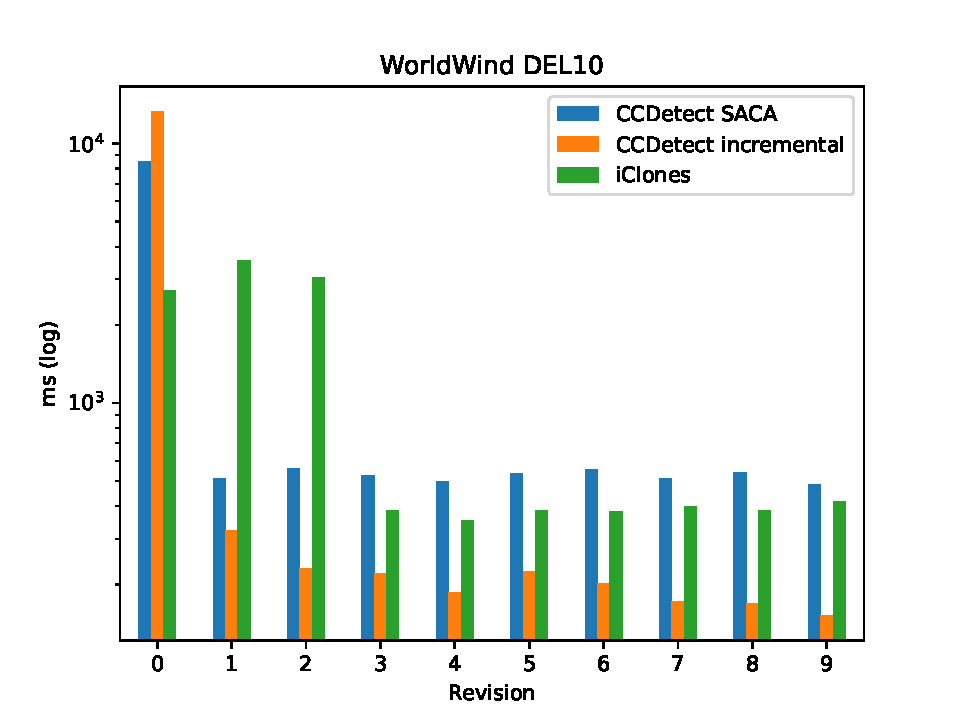
\includegraphics[width=0.49\textwidth]{figures/performancegraphs/WorldWind_DEL10.pdf}
        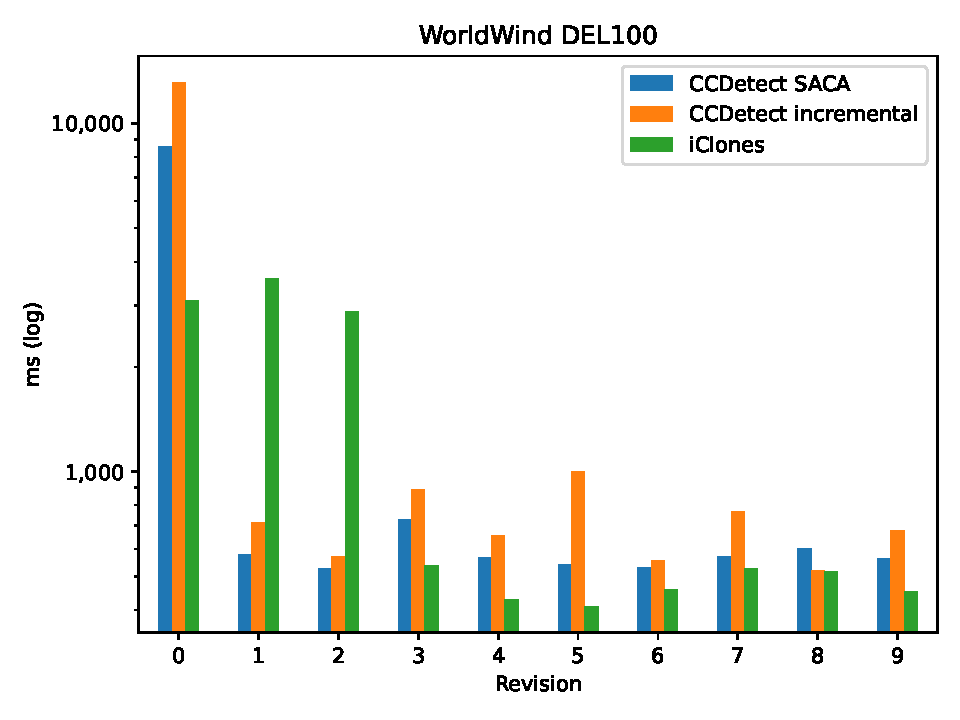
\includegraphics[width=0.49\textwidth]{figures/performancegraphs/WorldWind_DEL100.pdf}
        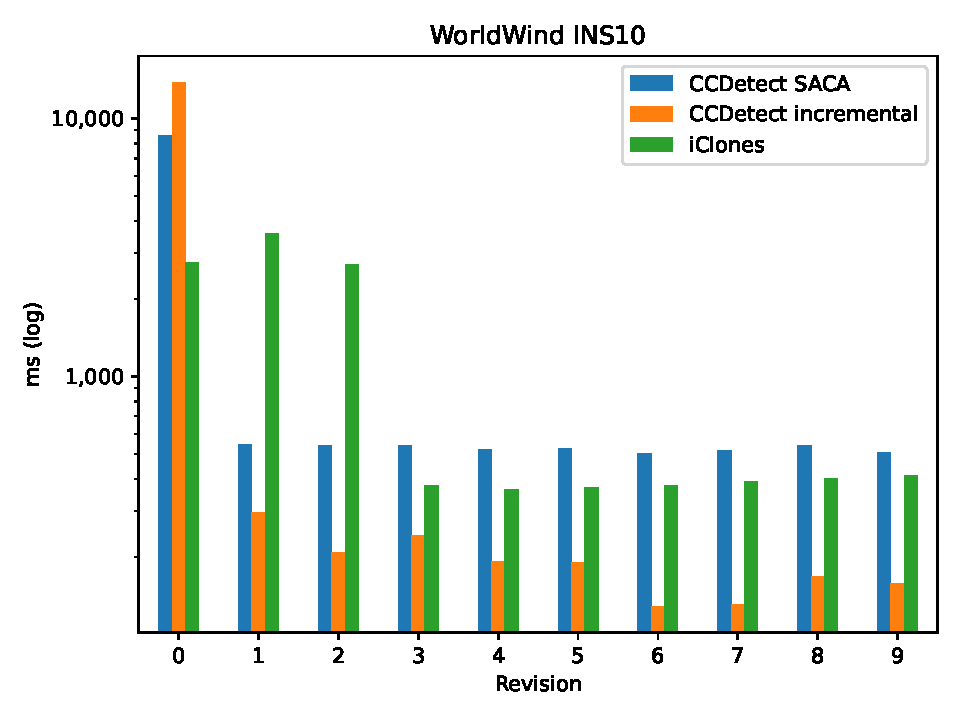
\includegraphics[width=0.49\textwidth]{figures/performancegraphs/WorldWind_INS10.pdf}
        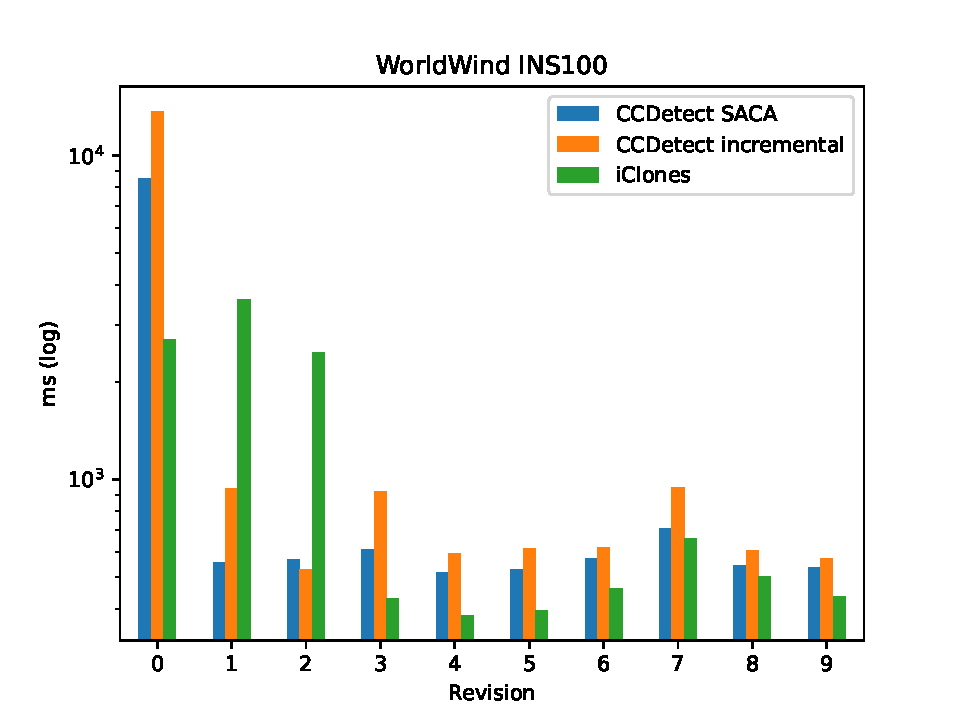
\includegraphics[width=0.49\textwidth]{figures/performancegraphs/WorldWind_INS100.pdf}
    \end{center}
    \caption{WorldWind performance benchmark}
    \label{fig:WorldWind}
\end{figure}

\begin{figure}[H]
    \begin{center}
        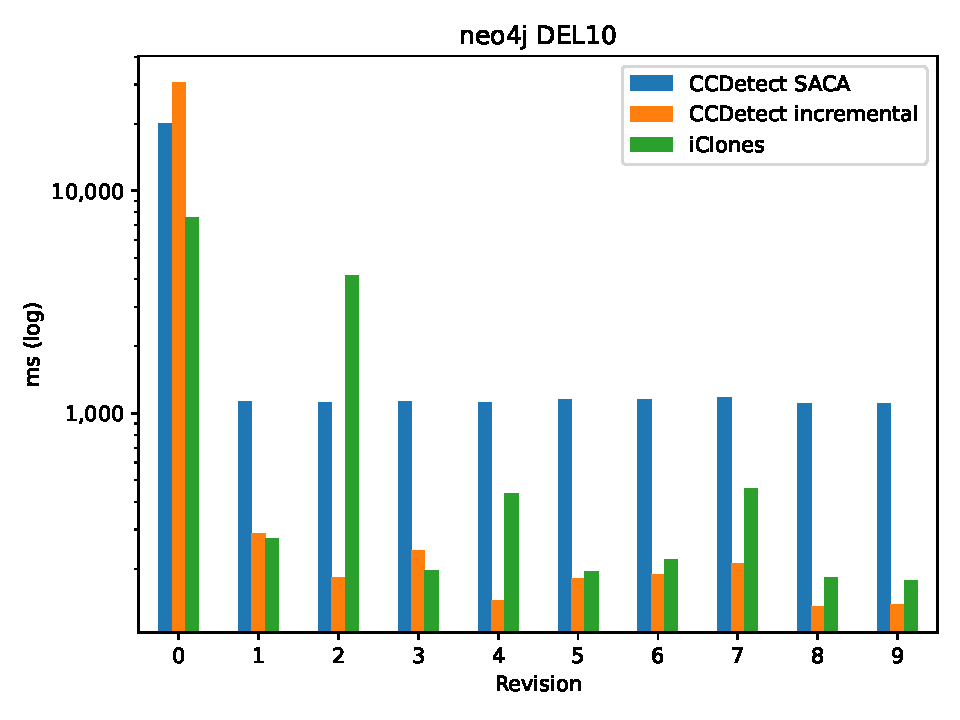
\includegraphics[width=0.49\textwidth]{figures/performancegraphs/neo4j_DEL10.pdf}
        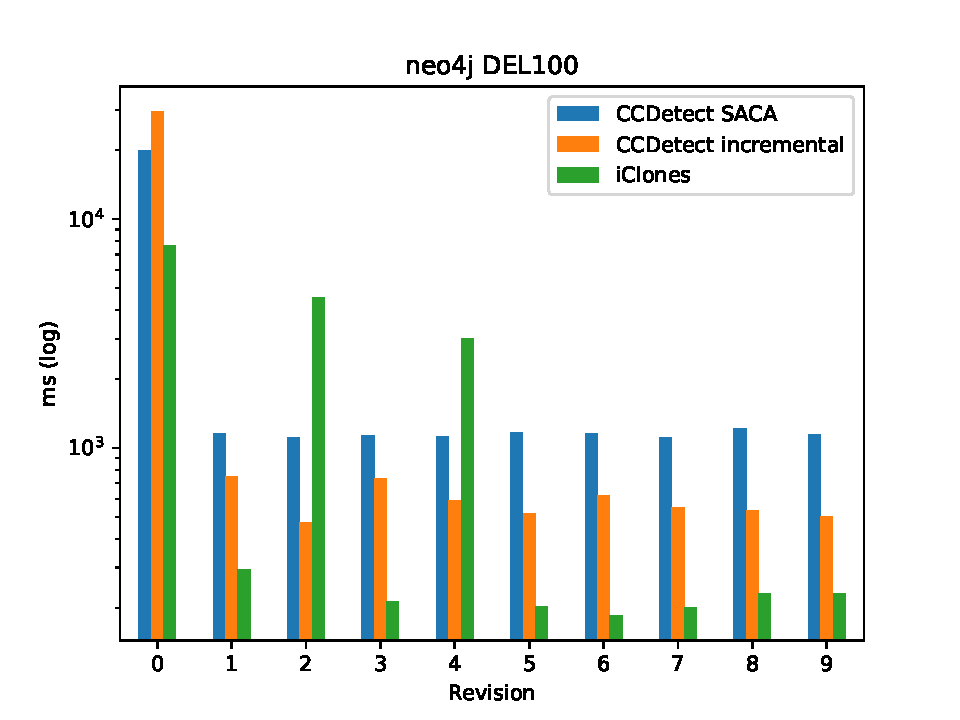
\includegraphics[width=0.49\textwidth]{figures/performancegraphs/neo4j_DEL100.pdf}
        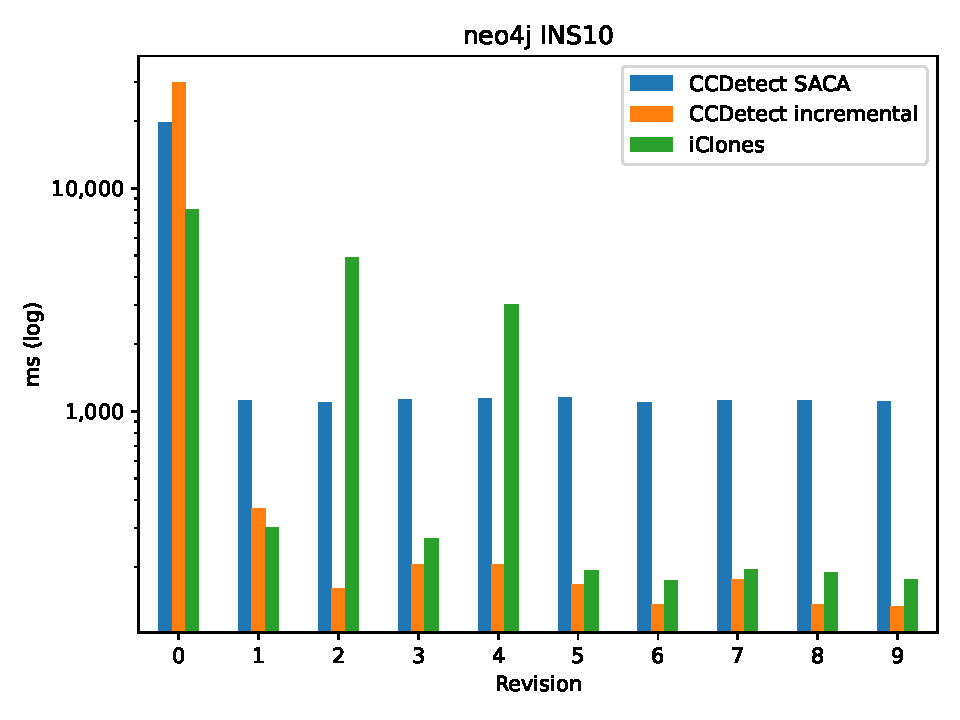
\includegraphics[width=0.49\textwidth]{figures/performancegraphs/neo4j_INS10.pdf}
        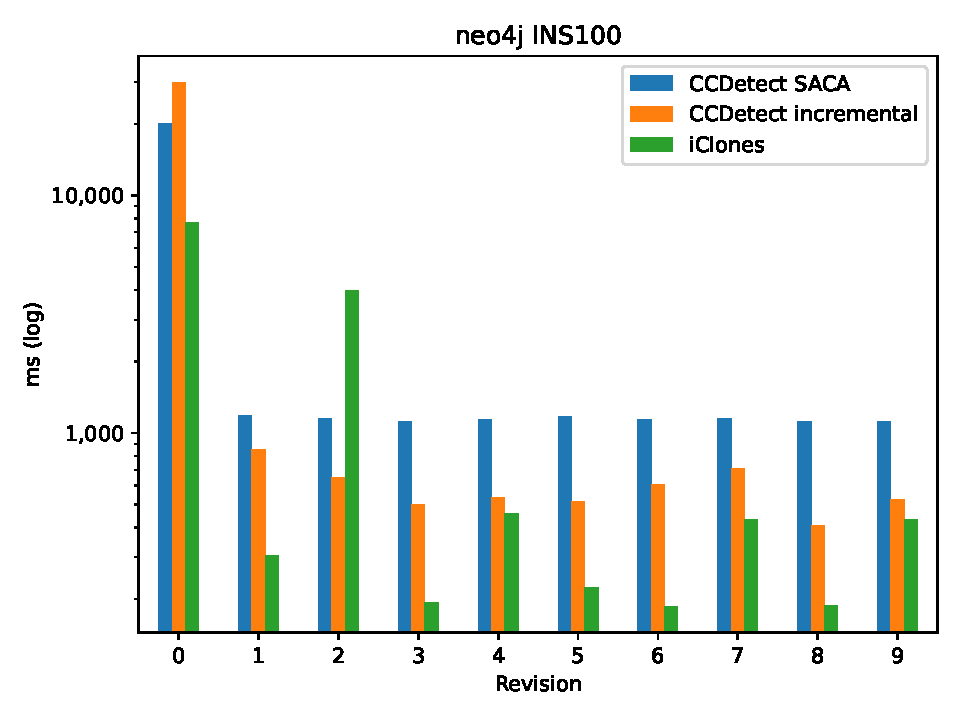
\includegraphics[width=0.49\textwidth]{figures/performancegraphs/neo4j_INS100.pdf}
    \end{center}
    \caption{neo4j performance benchmark}
    \label{fig:neo4j}
\end{figure}


\begin{figure}[H]
    \begin{center}
        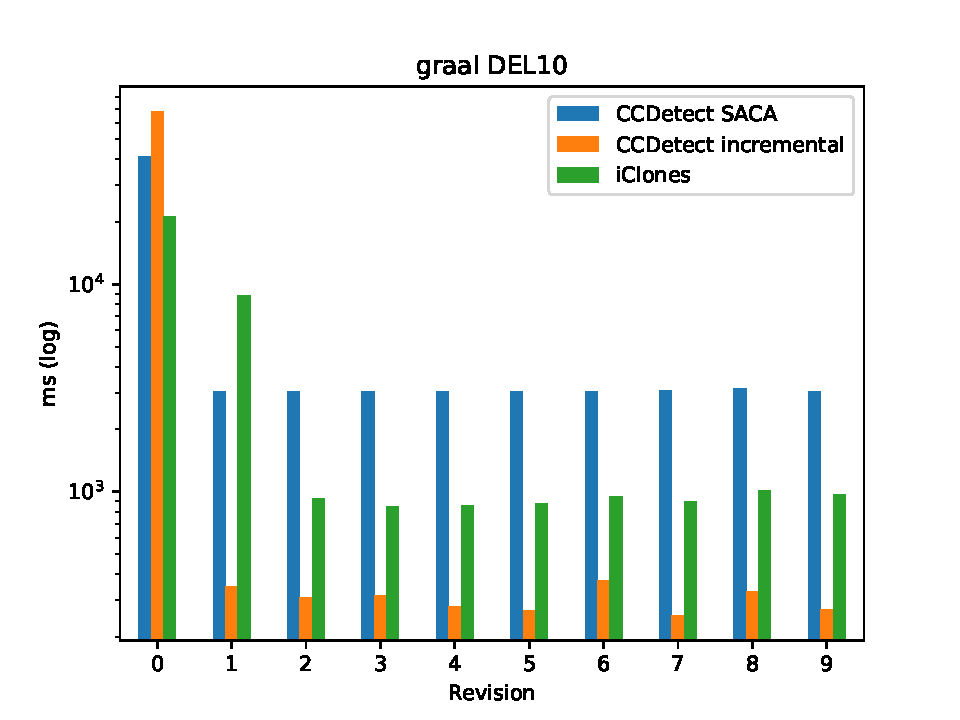
\includegraphics[width=0.49\textwidth]{figures/performancegraphs/graal_DEL10.pdf}
        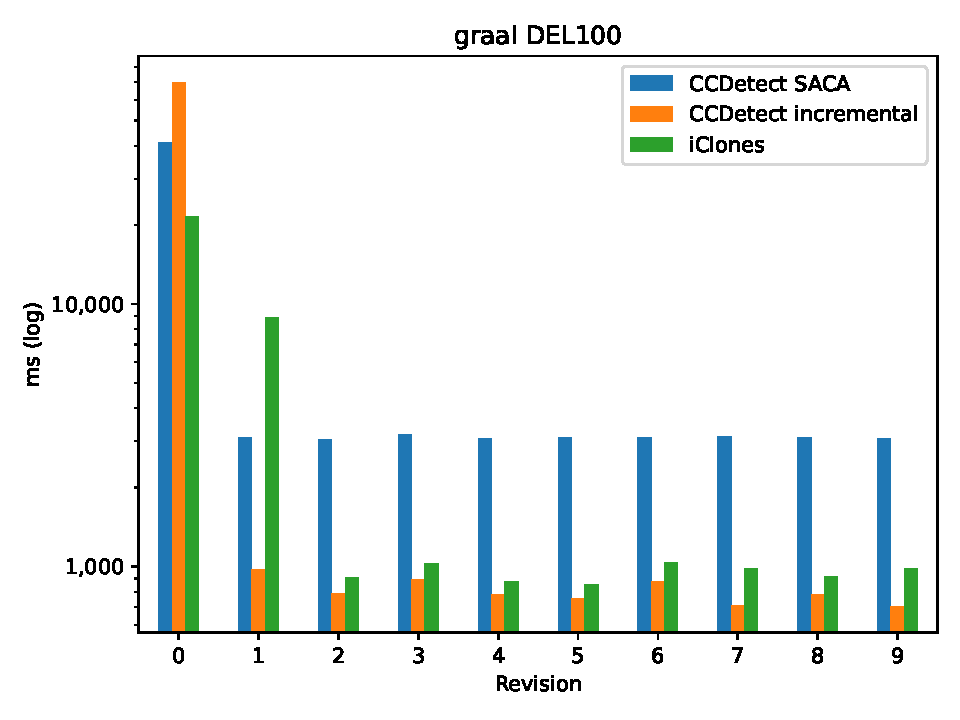
\includegraphics[width=0.49\textwidth]{figures/performancegraphs/graal_DEL100.pdf}
        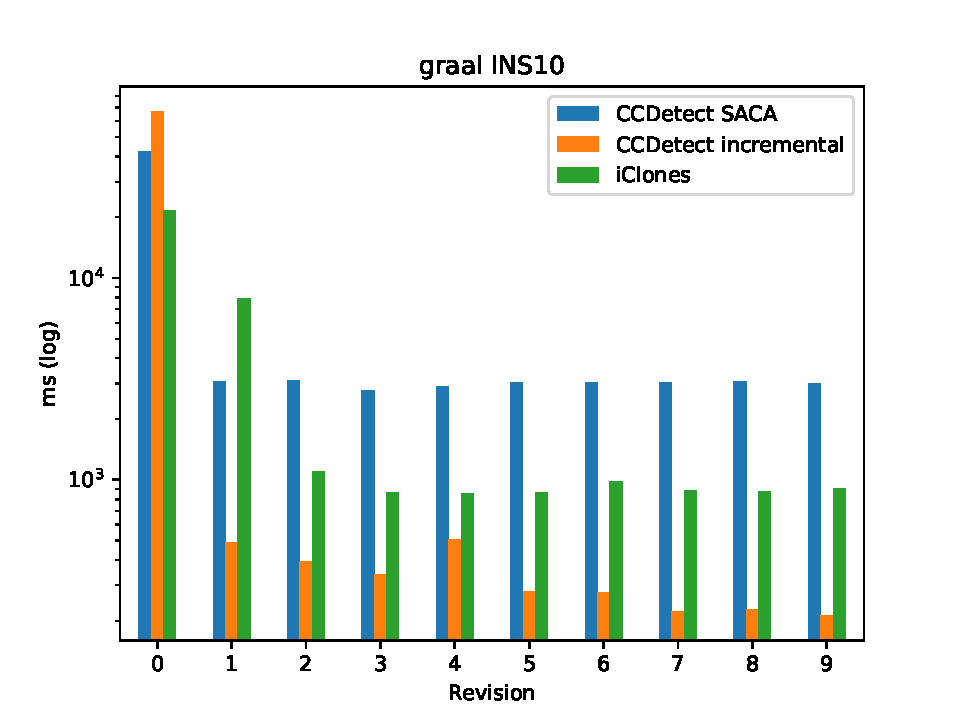
\includegraphics[width=0.49\textwidth]{figures/performancegraphs/graal_INS10.pdf}
        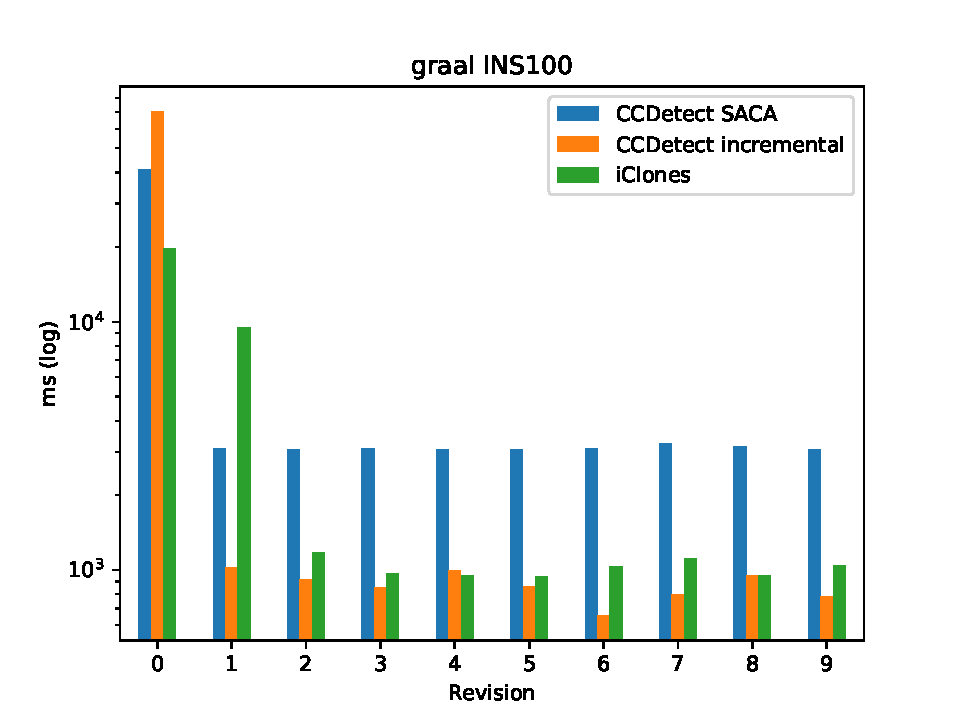
\includegraphics[width=0.49\textwidth]{figures/performancegraphs/graal_INS100.pdf}
    \end{center}
    \caption{graal performance benchmark}
    \label{fig:graal}
\end{figure}


\begin{figure}[H]
    \begin{center}
        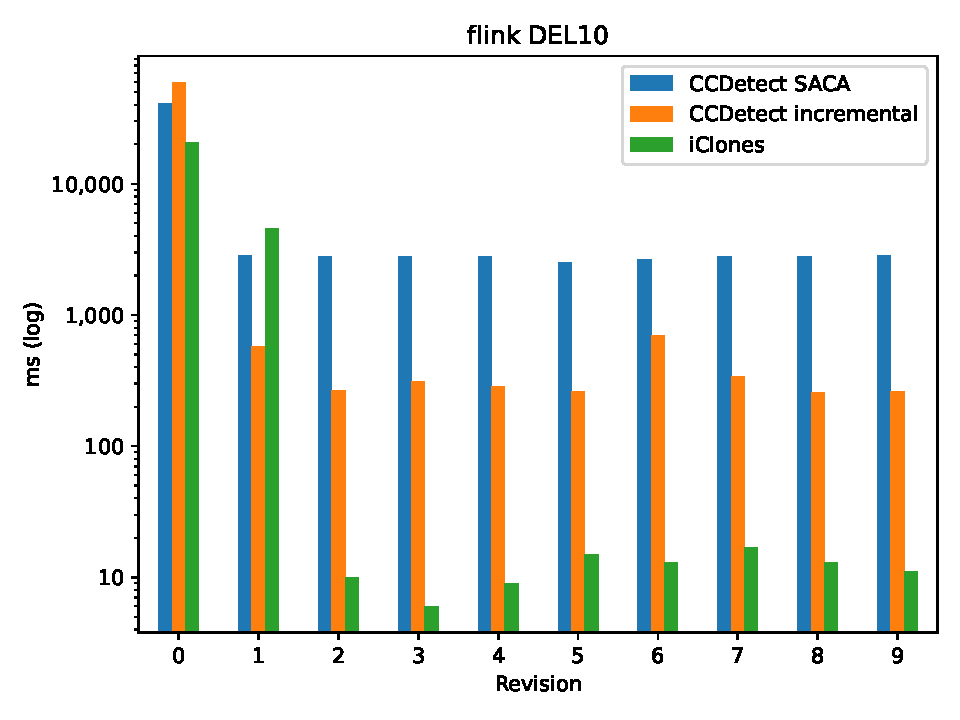
\includegraphics[width=0.49\textwidth]{figures/performancegraphs/flink_DEL10.pdf}
        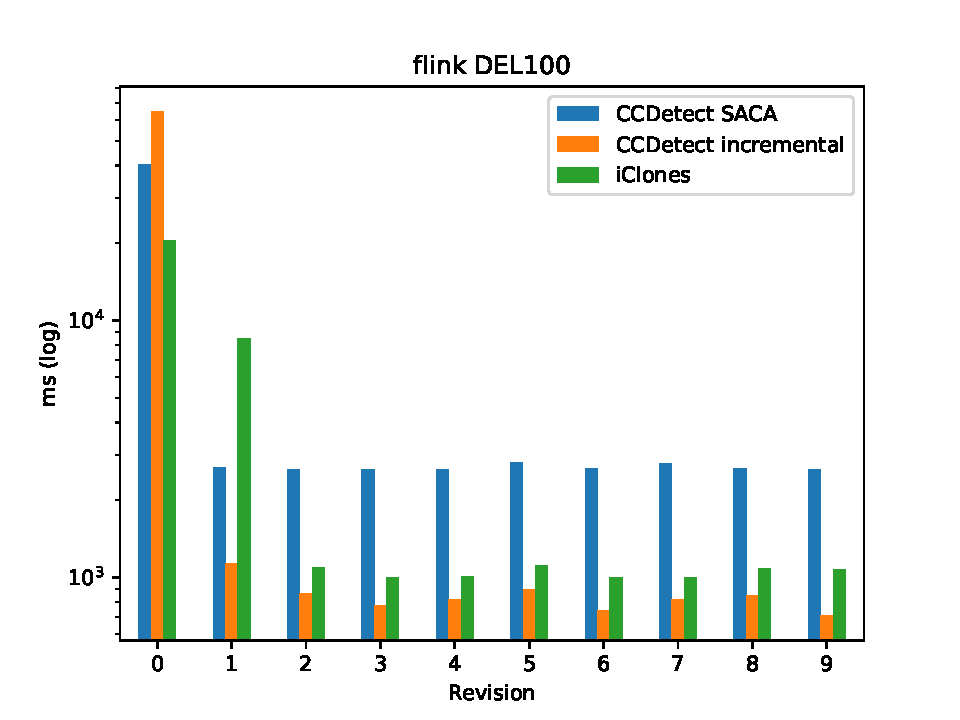
\includegraphics[width=0.49\textwidth]{figures/performancegraphs/flink_DEL100.pdf}
        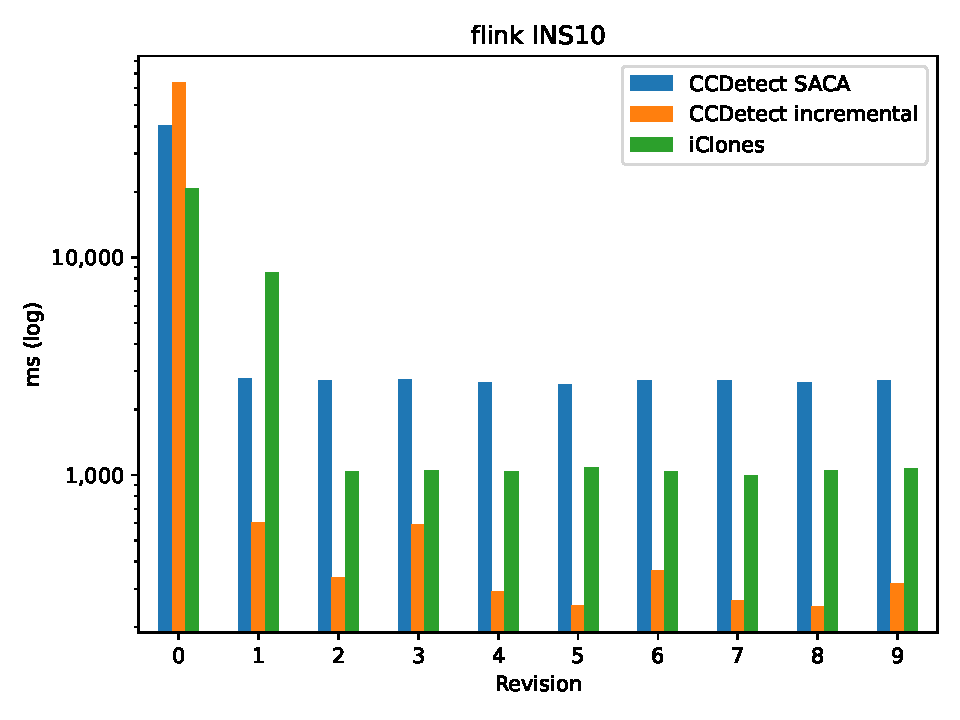
\includegraphics[width=0.49\textwidth]{figures/performancegraphs/flink_INS10.pdf}
        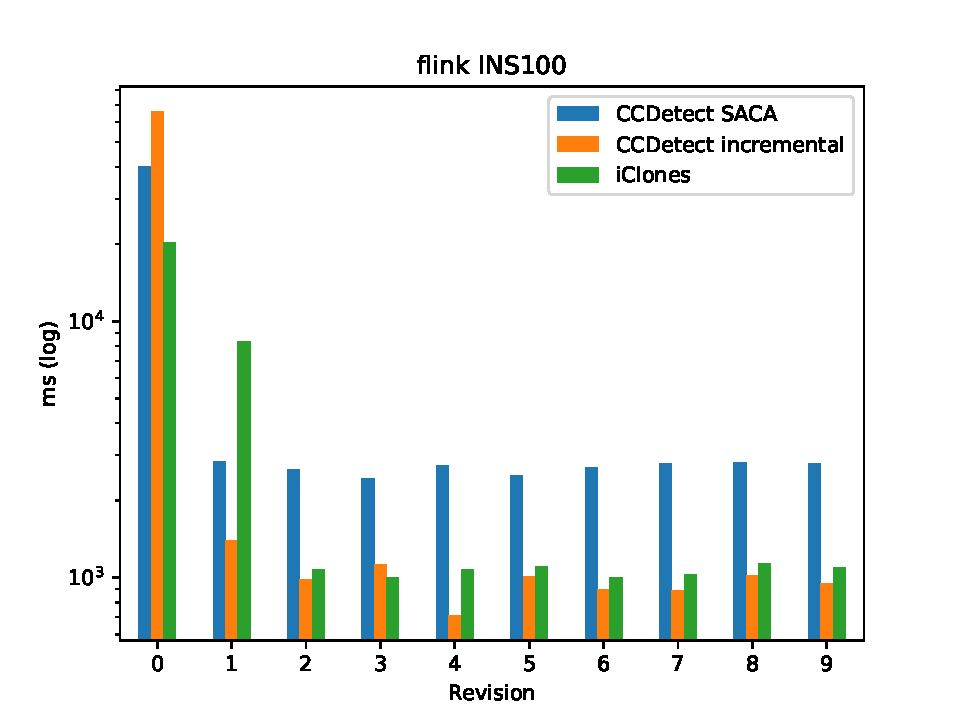
\includegraphics[width=0.49\textwidth]{figures/performancegraphs/flink_INS100.pdf}
    \end{center}
    \caption{flink performance benchmark}
    \label{fig:flink}
\end{figure}

\begin{figure}[H]
    \begin{center}
        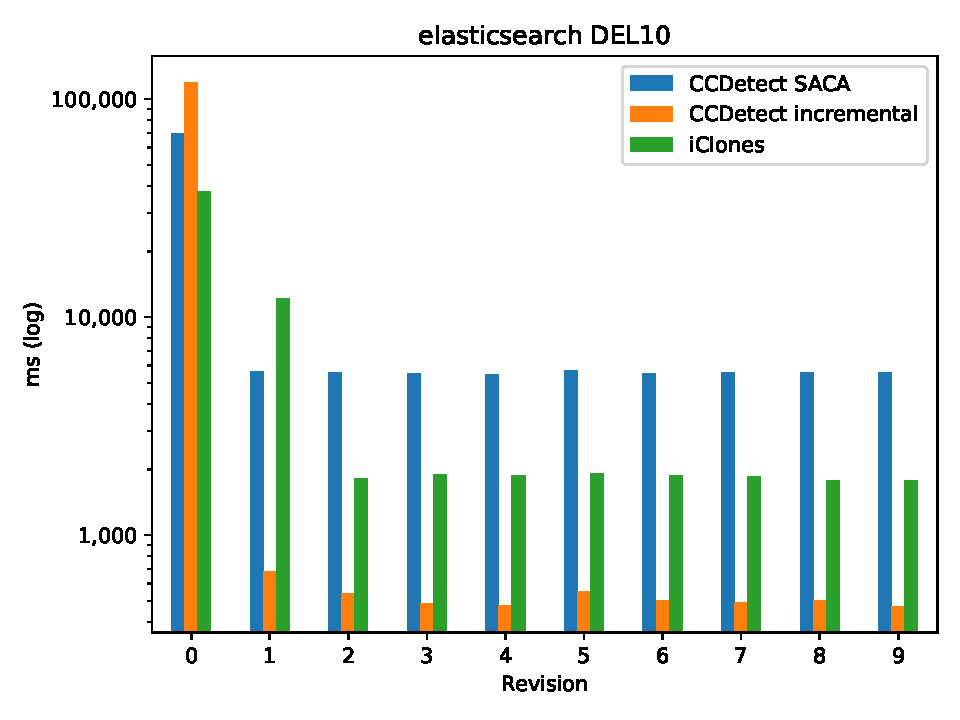
\includegraphics[width=0.49\textwidth]{figures/performancegraphs/elasticsearch_DEL10.pdf}
        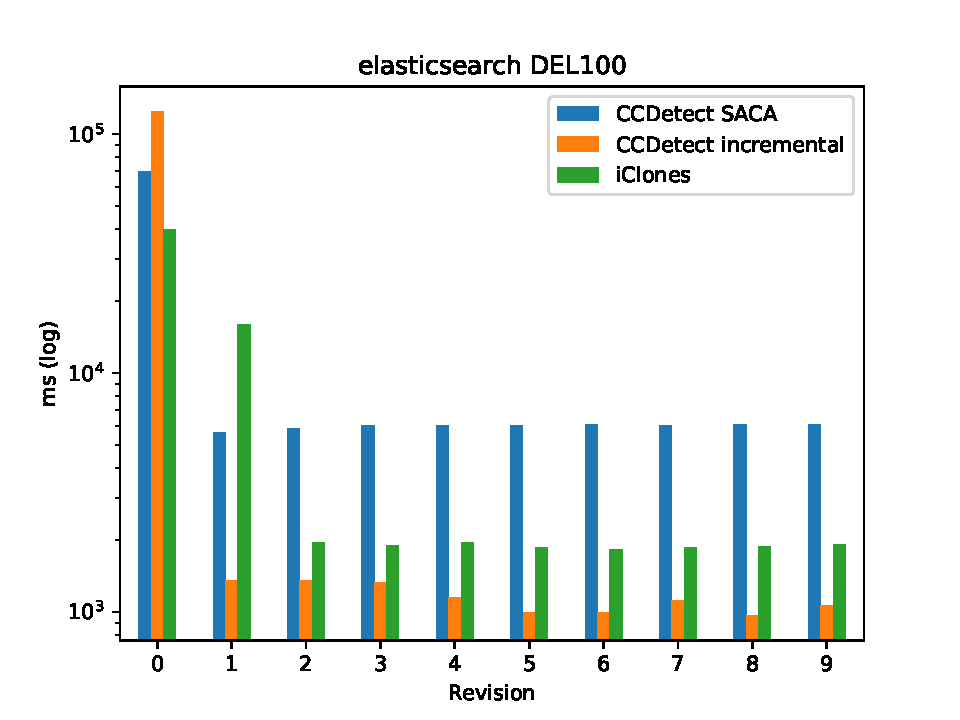
\includegraphics[width=0.49\textwidth]{figures/performancegraphs/elasticsearch_DEL100.pdf}
        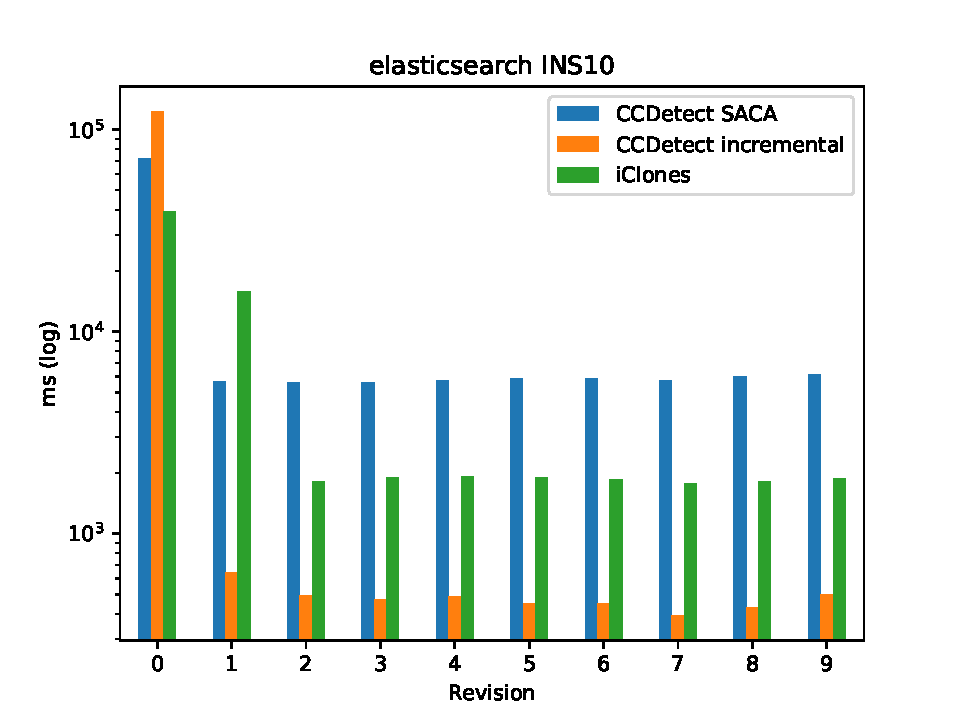
\includegraphics[width=0.49\textwidth]{figures/performancegraphs/elasticsearch_INS10.pdf} 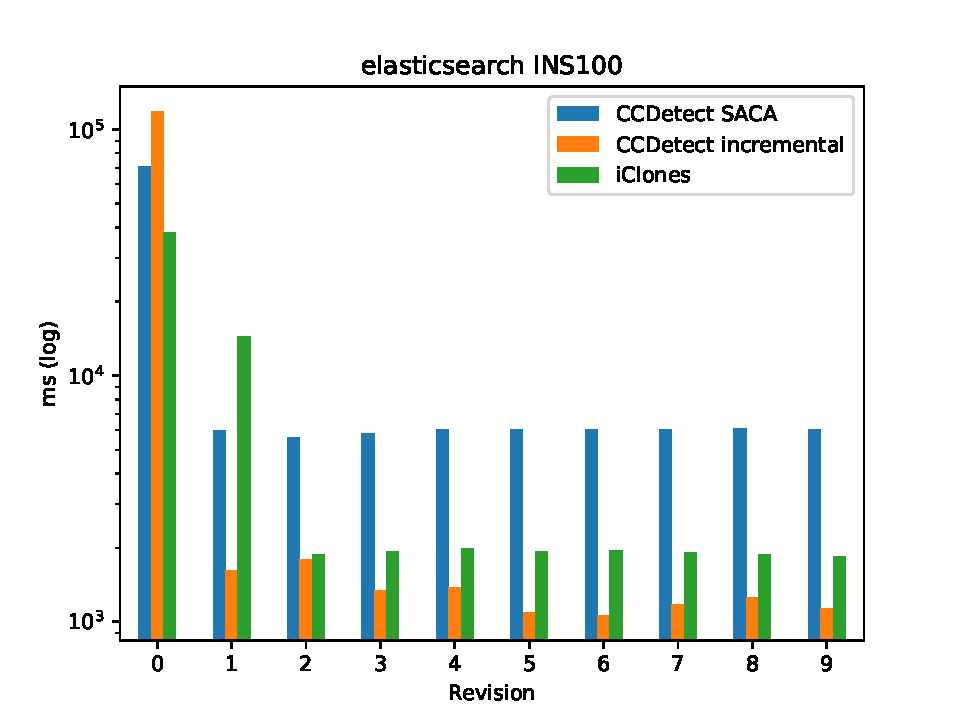
\includegraphics[width=0.49\textwidth]{figures/performancegraphs/elasticsearch_INS100.pdf} \end{center}
    \caption{elasticsearch performance benchmark}
    \label{fig:elasticsearch}
\end{figure}

\begin{figure}[H]
    \begin{center}
        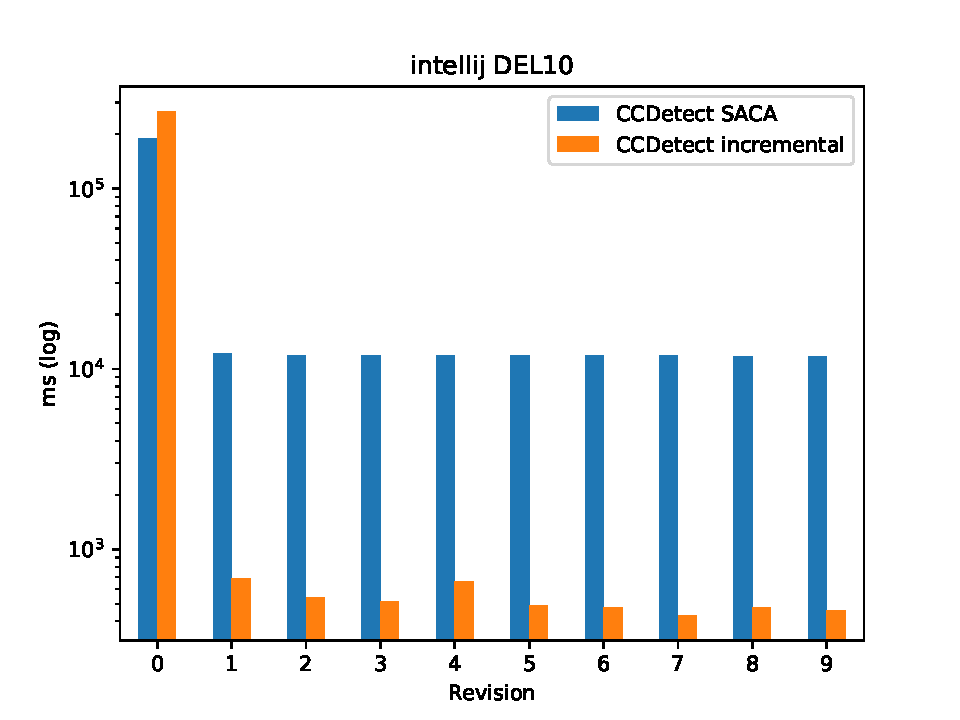
\includegraphics[width=0.49\textwidth]{figures/performancegraphs/intellij_DEL10.pdf}
        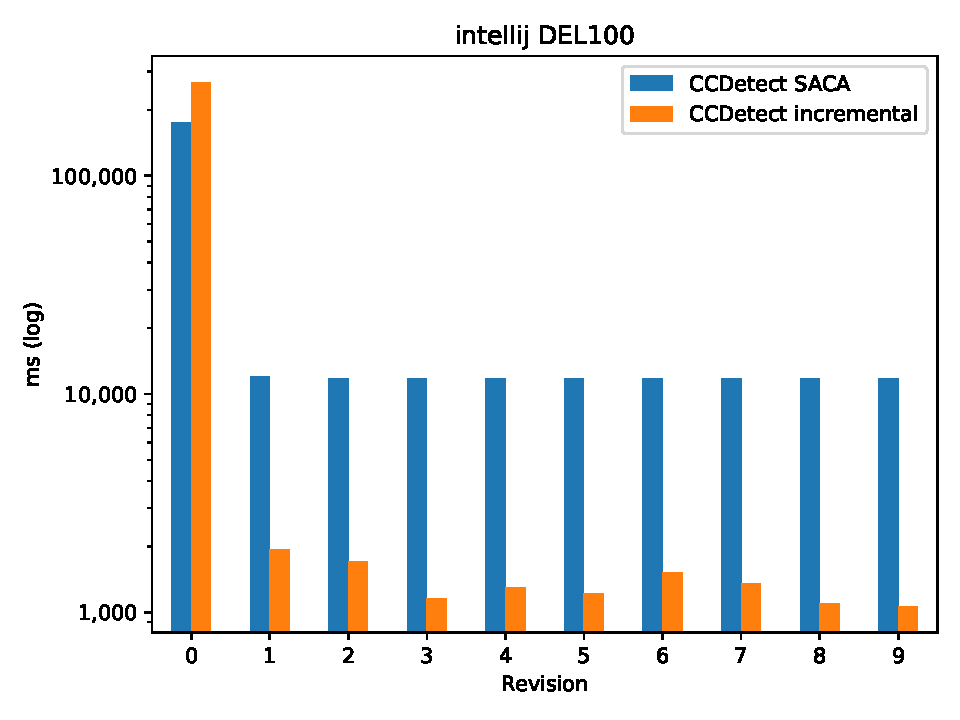
\includegraphics[width=0.49\textwidth]{figures/performancegraphs/intellij_DEL100.pdf}
        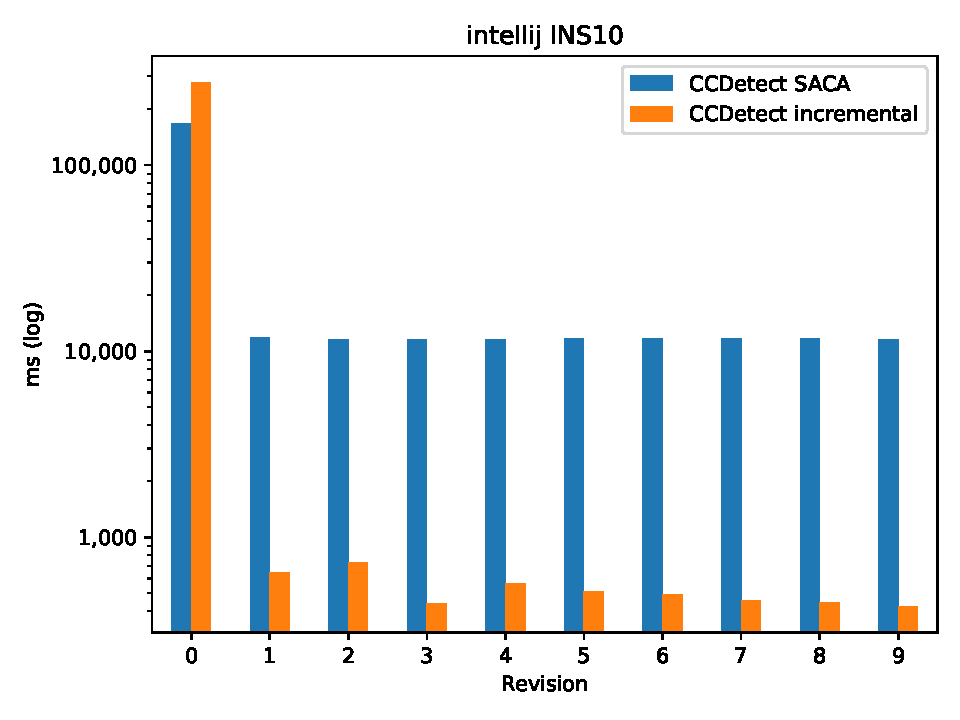
\includegraphics[width=0.49\textwidth]{figures/performancegraphs/intellij_INS10.pdf}
        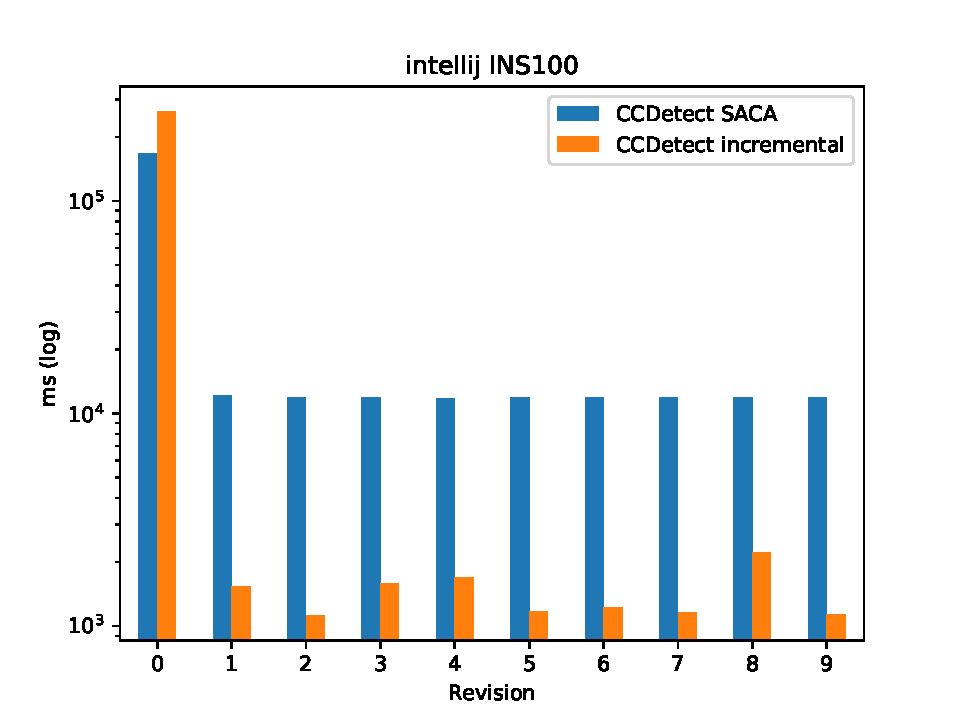
\includegraphics[width=0.49\textwidth]{figures/performancegraphs/intellij_INS100.pdf}
    \end{center}
    \caption{intellij-community performance benchmark}
    \label{fig:intellij}
\end{figure}

\section{Memory usage}

